% Rangefinding

\chapter{Rangefinding} % Main chapter title

\label{Rangefinding}

%----------------------------------------------------------------------------------------

\section{Overview}
 Rangefinding is the act of determining the distance between two things.
 
\subsection{The System}

\begin{figure}
	\centering
	\tikzstyle{vertex}=[circle, draw]
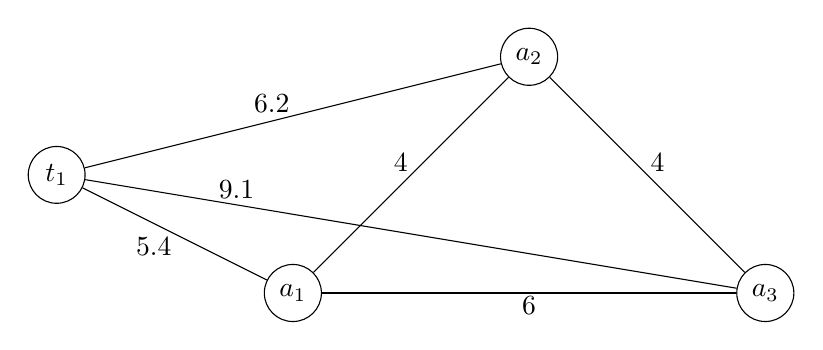
\begin{tikzpicture}[transform shape]
\node[vertex](a1) at (0, 0) {$ a_1 $};
\node[vertex](a2) at (3, 3) {$ a_2 $};
\node[vertex](a3) at (6, 0) {$ a_3 $};
\node[vertex](t1) at (-3,1.5) {$ t_1 $};

\begin{scope}[every path/.style={-}, every node/.style={inner sep=1pt}]
       \draw (a1) -- node [anchor=south east] {$4$} (a2);
       \draw (a2) -- node [anchor=south west] {$4$} (a3);
       \draw (a1) -- node [anchor=north] {$6$} (a3);
       \draw (t1) -- node [anchor=north east] {$5.4$} (a1);
       \draw (t1) -- node [anchor=south east] {$6.2$} (a2);
       \draw (t1) -- node [pos=0.2, anchor=south west] {$9.1$} (a3);
\end{scope} 
\end{tikzpicture}
	\decoRule
	\caption{An example network, showing 1 tag $t_1$ and 3 anchors $a_i$ and the reported distances between them. Note that each device calculates its own range to the other devices, which will be slightly different from the range calculated on the other devices. This is not shown on the diagram.}
	\label{fig:ExampleNetwork}
\end{figure}

The rangefinding subsystem is comprised of \textbf{nodes} in a network, each of which is capable of sending and receiving wireless signals.

Each node is either an \textbf{anchor} or a \textbf{tag}. Both tags and anchors use essentially the same hardware and code, but anchors are assumed to be stationary while tags are mobile. Stationary nodes are required so as to provide a consistent frame of reference for other nodes when calculating positions later on. More information on this can be found in Section~\ref{FrameOfReference}.

The rangefinding subsystem's purpose is to determine the distances between every pair of nodes in the network. With this data, the position calculation subsystem can then determine the positions of every anchor and tag in 3D space. An example 2D rangefinding network is shown in Figure~\ref{fig:ExampleNetwork}.

\subsection{Rangefinding}
Rangefinding is done wirelessly. The underlying concept is that if we precisely note the times at which we send and receive a signal, then -- since light travels at a fixed speed -- we can determine the distance the signal traveled, which is the distance between the nodes. 

The basic algorithm for the network is: 
\begin{enumerate}
	\item Each node broadcasts a message to every other node, and every node responds. 
	\item The time it took for the message to travel from one node to another and then back (minus the time spent processing the received messages) is calculated.
	\item With some simple math involving the speed of light the distance between the nodes is calculated. 
\end{enumerate}

This method of calculating range is known as \textbf{time-of-flight} (TOF).

Each node is comprised of a DWM1000, can send wireless signals, and an Arduino microcontroller.

\subsection{Requirements}
There are a number of useful characteristics a rangefinding system should have:
\begin{itemize}
	\item Ranges should be accurate and not very noisy.
	\item Ranges should be calculated at a high frequency. If they are not, then we cannot calculate positions quickly and moving objects will have their positions displayed inaccurately.
	\item The system should be able to cover a large area. 
	\item The system should be robust to nodes entering/leaving the network. 
\end{itemize}

It will be demonstrated how we sought to satisfy these criteria.

(TODO TALK ABOUT WHAT IS COMING UP IN THE REST OF THE CHAPTER)

\section{Time-of-Flight}
This section briefly covers the math behind time-of-flight range calculations. For more in-depth information, \parencite{DW1000UserManual} has a comprehensive write-up of the different ways wireless ranging can be performed as well as an error analysis.

\subsection{Propagation Time}
The goal behind time-of-flight is to measure the propagation time of a signal, $T_{prop}$. Once we obtain this, it is a simple measure to calculate the distance $d$ between the two nodes using the speed of light, $c$, with the following formula:

\[
	d = c T_{prop}
\] 

\subsection{Single-sided Two-Way Ranging}
\begin{figure}
	\centering
	\includegraphics[width=\linewidth]{Figures/BasicRanging.png}
	\decoRule
	\caption{Single-sided two-way ranging. Figure from \parencite{DW1000UserManual}.}
	\label{fig:BasicRanging}
\end{figure}

In the case where there are two nodes communicating with each other, \parencite{DW1000UserManual} states that one can calculate the time it takes a signal to propagate between them, $T_{prop}$, as:

\[
	T_{prop} = \frac{T_{round} - T_{reply}}{2}
\]

where $T_{round}$ and $T_{process}$ are the total durations between receiving and transmitting messages as can be seen in Figure~\ref{fig:BasicRanging}.

\subsection{Double-sided Two-way Ranging}

\begin{figure}
	\centering
	\includegraphics[width=\linewidth]{Figures/AsyncRanging.png}
	\decoRule
	\caption{Double-sided two-way ranging with three messages. Figure from \parencite{DW1000UserManual}.}
	\label{fig:AsyncRanging}
\end{figure}

Because the clocks of two nodes may not pass time at the same rate (clock skew), the above equation will suffer from significant error. This is because processing times far dwarf the time it takes a signal to propagate. \parencite{DW1000UserManual} presents, without proof, the following equation for more accurate rangefinding:

\[
	T_{prop} = \frac{T_{round1}  T_{round2} - T_{reply1} T_{reply2}}{T_{round1} + T_{round2} + T_{reply1} + T_{reply2}}
\]

where $T_{round1}$, $T_{round2}$, $T_{reply1}$, $T_{reply2}$ are the durations between sending and receiving messages as seen in Figure~\ref{fig:AsyncRanging}. An independently derived proof of this equation can be found in Appendix~\ref{AsyncProof}.

Because the ranging has two rounds, after the initial calculation of range we can calculate a new range value for every single following transmission by re-using the last timestamps received for the beginning of the next round.

\section{Wireless Communications}
At the start of the project, it was determined that a technology would need to be chosen to handle wireless communications for ranging purposes. A number of options were considered. The ideal technology would:
\begin{itemize}
	\item Be inexpensive.
	\item Have good range for in-door use.
	\item Allow for extremely precise measurements of time. Due to the speed of light, a nanosecond of error in timing calculations would lead to approximately 30cm of error in the calculated distance.
	\item Be small. As tags are attached to cellphones, they must be small.
\end{itemize}

\subsection{Bluetooth in Phones: A Failed Approach}
Originally, the goal was to use Bluetooth for ranging. The reason for this was that Android cellphones, which usually have Bluetooth transceivers, could be used for tags and anchors. This would save a large amount of time, as cellphones include batteries, are easy to program, and almost everyone has one (which would make letting people use our project as easy as downloading an app). We would just need to put a few phones running our app around a room, and we'd get ranging. Others, such as \parencite{BluetoothIndoor}, were able to use Bluetooth to form indoor positioning systems.

Unfortunately, it became clear early on that Bluetooth -- specifically, Bluetooth used on Android cellphones -- was not suitable. 

There were two ways to use Bluetooth for ranging, and we checked the viability of both: 

\begin{itemize}
	\item RSSI (received signal strength indicator), which is essentially a measure of how strong a received signal is. Because signal power drops off with the square of distance, RSSI can be used to determine distance from a cellphone. Indeed, there this is a cellphone app to do just that on the Google Play Store. Measurements showed that this was method had very low range, was very noisy (power levels varied wildly), and had a large latency between measurements. As well, RSSI values are not standard among cellphones, requiring many calibrations for each model of phone used. Due to these factors, it was determined that using RSSI for distance measurements was not well suited for the fine-grained location tracking this project sought. 
	\item Time-of-flight measurements. Experiments showed that the time it took to send a Bluetooth message itself through the Android OS suffered massive variance of milliseconds (ADD IN APPENDIX CITATION WITH OUR CODE?), which would lead to 300 km of error in calculated distances! Android does not have any guarantees on timing, and does not allow low-level programming access to its internals. This method was proven unworkable.
\end{itemize}

With all the avenues to use Bluetooth exhausted, the idea of using phones and their Bluetooth transceivers was rejected.

\subsection{Ultra-wideband and the DWM1000}
After doing some research, we discovered the Decawave DWM1000 ultra-wideband transceiver. This chip is advertised as specifically being suited for ranging applications. It uses ultra-wideband technology rather than Bluetooth, Wi-Fi, or similar technologies.

Ultra-wideband, in contrast to Wi-Fi and other radio technologies, occupies a large bandwidth and transmits information via high-bandwidth pulses. Ultra-wideband is suited to tracking applications due to its resistance to multipath propagation, a phenomenon where signals reflect off of surfaces and thus reach the antennae via multiple paths (causing interference). An in-depth look at ultra-wideband is beyond the scope of this report, but interested readers might look more at (INCLUDE SOURCES HERE!!!).

The DWM1000 is advertised as:
\begin{itemize}
	\item Allowing one to locate objects with up to 10cm accuracy.
	\item Having a range of up to 290m.
	\item Having a data rate of up to 6.8Mb/s.
	\item Having a small physical size. 
\end{itemize}

As well, there was an already an open source library written to use it with an Arduino, which would allow us to quickly prototype with the chip and ensure it would fit for our application.

Because these qualities satisfied our requirements, the DWM1000 was chosen for the foundational technology of the ranging part of the project. 

\section{Design of the Hardware}
The hardware design for tags is an Arduino Pro Mini 3.3V connected to a DWM1000 over a PCB. 

\subsection{The Microcontroller}
To interface with the DWM1000, a microcontroller was needed. The Arduino Pro Mini 3.3V was chosen because:
\begin{itemize}
	\item Group members had previous experience with programming Arduinos.
	\item It was inexpensive.
	\item It worked off of 3.3V power, which was what the DWM1000 required. This obviated the need for voltage stepping.
	\item It is capable of floating point math, which is useful for asynchronous two-way ranging. As well, barely any processing power or RAM was perceived to be needed (this was not quite true). Each microcontroller only needed to hold a small number of timestamps, so the small amount of memory and slow processor was not important.
	\item It has a small physical size. As tags are attached to cellphones, they must be small.
	\item Batteries would not be needed to power tags, since power could be delivered via USB from the cellphone. This further simplified the design and kept costs low.
\end{itemize}

The only real downside of the Pro Mini was that it required a lot of soldering. 

\subsection{The PCB}
Several designs were considered for the PCB connecting the Arduino and DWM1000. An important factor was size. A PCB was constructed only for the tags, and anchors - which did not need to be reduced in size - were left in breadboard form in order to save costs and time. Making alterations to the PCB design to allow for a barrel jack power adapter (the only distinguishing feature between tags and anchors) would, however, have been extremely simple.

The first design idea we tried was to place the Arduino and DWM on top of each other, resulting in the smallest possible size. See (INSERT FIGURE HERE). However, the physical dimensions of the two components made this impossible. The other possibility was to place each component on opposite sides of the PCB (INSERT FIGURE HERE), but the Arduino's design demanded breakout headers to solder it into the board, which meant the PCB had to have holes drilled. This essentially ran into the same problem as with the original.

The second idea was to make two PCBs. The Arduino would connect to a PCB above it, and that PCB would connect to a board above it with the DWM1000 it. Because it was layered, the pins connecting the layers could be arranged such that the Arduino and DWM1000 were essentially above each other (but without interfering with their pins, as before). See (INSERT FIGURE). In the end, this design was abandoned because the breakout pins would add to much vertical length, it was expensive, and because it was much more complex to design.

As such, the end design required the Arduino and DWM1000 to be spread out over the board, resulting in the PCB being quite long and narrow. The PCB design was done in Eagle and ordered from PCBWay. The result can be seen in (INSERT FIGURE).

\section{Arduino Software}
The software to control the DWM1000 was written in C++ in Arduino IDE. The basic code to control the DWM1000 (handling memory address constants, communication with it via SPI, and a few high-level functions like send/receive) was freely available in Thomas ``thotro'' Trojer's \texttt{arduino-dw1000} library. The library served as the foundation of our code to network the devices.

\subsection{Networking Basics}

Each node in the network broadcasts in a round robin fashion, with a small break after each node has transmitted. As part of the transmitted message, the node transmits the timestamp of when it is sending the message, a list of the timestamps when it last received a communication from every other node in the network, and a list of the last computed ranges to the other nodes. Every other node in the network will receive this information and use it to compute a new range to the node in question. Thus, every node in the network receives complete range information for the whole network.

The DWM uses 40 bits (5 bytes) for its timestamps. The Arduino internally represents these as 64-bit integers (the last byte being meaninless), but transmits them as 40 bit (5 byte) numbers.

Every node in the network has a pre-determined ID, which is set when it the code is programmed onto the device. A single byte is used for this ID to save as much space as possible, though the code could easily be modified to support longer IDs if the devices were to be mass produced. Alternately, something like DHCP could be implemented. As there are only 7 devices currently operational, our project only uses IDs 1 through 7, though the IDs do need not be consecutive. ID 255 is a special dummy value used in the code and should not be selected for use with an actual device.

Communications between the Arduino and the DWM1000 are handled through SPI. When the DWM1000 receives a message, it triggers an interrupt on the Arduino, which can then obtain the received data through SPI.

\subsection{Communications Timing}

\begin{figure}
	\centering
	\begin{tikzpicture}

\def \n {6}
\def \radius {3cm}
\def \margin {11} % margin in angles, depends on the radius

\begin{scope}[auto, every node/.style={draw,circle,minimum size=2em,inner sep=1},node distance=2cm]
\foreach \id [count=\s] in {1, 2, 5, 8, 10, 255}
{
  \node at ({360/\n * (\s - 1)}:\radius) {$\id$};
  \draw[->, >=latex] ({360/\n * (\s - 1)+\margin}:\radius) 
    arc ({360/\n * (\s - 1)+\margin}:{360/\n * (\s)-\margin}:\radius);
}
\end{scope}

\end{tikzpicture}
	\decoRule
	\caption{Transmission order of a network composed of five devices with IDs 1, 2, 5, 8, and 10. Note they transmit in order, and there is a dummy ID of 255 which serves as a marker for the end of the round.}
	\label{fig:TransmissionOrder}
\end{figure}

In order to maximize the operating frequency of the system and provide as smooth a visual experience as possible on the phone, we want to minimize the amount of time a node is not transmitting. In order to do this, it was decided that nodes should transmit in order of their ID in a round robin fashion. A round of transmissions are performed, each node transmitting once, and then it repeats. When one node receives a transmission, it checks to see if it is its turn and then transmits as soon as it can.

This round robin ordering is done by creating an ordered array of IDs in the network. When a transmission is received, the network increments the index of the next expected device to transmit by one. A device can tell whether it should transmit by checking to see if its ID is equal to the ID of the next expected node to transmit. If so, it transmits. 

The downside to this approach is that if any transmission were to be lost, for example by interference or electrical noise, the network would grind to a halt as it waits for a message that is never going to come. A solution to this is to include a timer that tracks a window in which a message should be received. If it takes too long to receive a message, the device was assumed to have to failed to transmit for some reason and the next device will take their turn and transmit.

To help the network be more robust, for example if one node has a clock that runs faster than the others (making it think a transmission is late when it is not), the network assumes whatever device last transmitted was right in doing so, and sets the index of the next node to transmit in the ordered array as being one higher than it.

This approach also raises the question of how new nodes will join the network if a node is constantly transmitting. To solve this, a small delay is added at the end of each round. When a device wishes to enter the network, it waits for the end of a round, and then does a transmission in this added space. This transmission lets all devices know it is part of the network, and they will add it to their ordered lists of IDs appropriately. 

In the code, this delay at the end of the round is implemented by adding a dummy node with the ID of 255 (the highest ID possible with one byte) to the network. The nodes will wait for a transmission from it at the end of each round, but it will never come, at which point the round starts over with the lowest ID transmitting. An example ordering can be found in Figure~\ref{fig:TransmissionOrder}.

An unsolved issue here is what happens when the transmission to join the network is sent and it is not received. This will cause the joining device to have a wrong order, and it will transmit at the same time as another device every round. Since the chances of this happening are quite low and could be solved by resetting the joining device, this is not dealt with. A possible solution to deal with this would be having the receiving device check the responses of all the other nodes to make sure they all received its transmission, and, if they have not, then to retransmit in the space at the end of the round until they do.

Code for this logic can be found in the \texttt{loop} function of Appendix~\ref{ArduinoCode}.

\subsection{Range Information Protocol}
The protocol for a transmission from a node is as follows:

\begin{itemize}
	\item 1 byte for the ID of the transmitting node.
	\item 5 bytes for the timestamp of the sending of the message.
	\item For each device the transmitting node has knowledge of:
	\begin{itemize}
		\item 1 byte for the ID of the device
		\item 1 byte for the shared counter (used to detect lost transmissions)
		\item 5 bytes for timestamp of last received message from the device
		\item 4 bytes for last calculated range	
	\end{itemize} 
\end{itemize}

Parsing a received message and updating range values from the parsed data is fairly straightforward. The code in question can be found in the \texttt{parseReceived} function in Appendix \ref{ArduinoCode}.

\subsection{Calculating a Delay}
\label{CalculatingADelay}
As part of the time of flight calculation, a timestamp is needed for when the message was received and for when the reply was sent. The DWM1000 does not offer a way to automatically set the time upon transmission, but does offer the ability to set a time when a message will be transmitted in the future. This timestamp can then be embedded in the message itself.

Ideally, this delay is short. However, if the delay is too short, the Arduino will not be able to transmit the data the DWM1000 should send before the timestamp is passed. This causes a silent error, and the DWM will not transmit anything. As well, the delay specified is not the delay at which the DWM1000 will begin transmitting, it is the delay that the DWM1000 will begin transmitting the data itself. There is a ``premable'' sent before any transmission to allow the other devices in the network time to wake up and begin sniffing the air and know a message is coming. This time to send the preamble lasts quite a long time (approximately 1 microsecond per symbol in the problem (ADD CITATION HERE), which adds up to almost 2 ms). This was the most difficult to solve bug that was encountered in the design of the system.

In the code, the delay before we can transmit is the sum of the:
\begin{itemize}
	\item Number of symbols in the preamble $\times$ 1\si{\micro\second} (128 is the value used here, though the DWM offers a choice of preamble length)
	\item Time required to calculate and send the timestamp using SPI, about 1000\si{\micro\second} (empirically determined)
	\item Bytes of data to transmit $\times$ 4.5\si{\micro\second}, or 85 $\times$ number of devices in the network besides this one (empirically determined)
\end{itemize}

Adding in a fudge factor of about 200\si{\micro\second}, the delay we use in code for 6 devices is roughly 1800 \si{\micro\second}.

It is important to minimize this delay so to increase the maximum frequency the system can update ranges at. The tradeoff of having a short preamble versus a long one is that a long preamble means there is less chance of a transmission being missed, at the cost of using more power and taking longer to send. The value of 128 was chosen as it was the smallest possible. Tests indicated that transmissions were not being lost enough to matter with such a short preamble.

\section{Calibrating}
DWM1000s need to be calibrated to give correct distances due to the differences in hardware. There are a number of factors affecting the DWM1000, such as temperature. Some of these factors are controlled for in software in the arduino-dw1000 library. For a detailed overview of the possible errors and how to correct for them, consult the INCLUDE SOURCE HERE IT WAS A PDF ON THE SITE I READ.

The primary factor which could not be controlled for by Decawave is the antenna delay. The capacitance of the hardware the DWM1000 is hooked up to can cause nanosecond-level delays in transmission (in experiments, it was found that this could cause up to several meters of error incorrectly configured). This is a constant, and is determined empirically. The antenna delay for the tags is the same and was found to be INSERT NUMBER HERE THAT WE FOUND, and the antenna delay for the anchors is roughly the same and was found to be INSERT NUMBER HERE.

These constants required a slight tweak to the DWM1000 library. INSERT LINK TO SOURCE CODE OF OUR CHANGED VERSION HERE.

\section{Operating Frequency Analysis}
\label{OperatingFrequencyAnalysis}
In order to estimate the operating frequency of the rangefinding subsystem -- that is, how many times we can get the range from all devices to a single device per second\footnote{It should be noted that this definition of operating frequency is somewhat misleading and calculates a minimum operating frequency. Because each pair of devices compute their range twice, once on each device at different points in the round, the true operating frequency of the system will be higher on average. The analysis here does not take this into account. 

In the best case scenario, this will almost double the system frequency. In the worst case scenario, where two devices are next to each other in the transmission order in a large network, the system operating frequency will barely increase. The figures given for operating frequencies will thus give a range from the minimum by the definition here to twice it.} -- we see that the frequency will be the inverse of the time taken to complete one round (the system performs one range update per device per round), assuming no lost transmissions. That is,

\[
 	f_{op} = 1/T_{round}
\]

The time it takes a round is equal to the time it takes the devices to each parse a received message and transmit a message. Determining the time it takes to transmit a message is a little tricky to calculate due to the requirement to include the delay before the message is sent. A rough estimate of the time it takes to do a round of transmissions is:

\[
	T_{round} =  N(T_{device} + T_{prop}) + T_{end}
\]
where $N$ is the number of nodes in the network (the 4 anchors and 3 tags that were made make 7), $T_{device}$ is the time it takes a device to fully receive and transmit, $T_{prop}$ is the time it takes the message propogate (this will not be constant, but it is so small as to be ignorable in this analysis), and $T_{end}$ is the duration of the pause at the end of the round. 

We can estimate $T_{device}$ as

\[
	T_{device} \approx T_{rx} + T_{tx} + T_{txDelay}
\]
where $T_{rx}$ is the time it takes to parse a received message (7-8 ms empirically), $T_{tx}$ is the time it takes to create the packet to send to the DWM1000 (1-2 ms empirically), $T_{txDelay}$ is the delay before the ranging packet can be sent (calculated in Section~\ref{CalculatingADelay}, about 1800 \si{\micro\second}).

Putting it all together, the equation estimating the operating frequency of the system is:
\[
	T_{round} \approx N(T_{rx} + T_{tx} + T_{txDelay}) + T_{end}
\]

$T_{end}$ is implemented in the code as a dummy device which the network will never receive a message for, allowing it to expire. Perhaps unintuitively, it is not actually equal to the time it takes a normal device to be rejected. This is because, when the round ends, it will not have transmitted anything, meaning that the time it takes to parse a received message will be 0 from it and the next round will start as soon as the first device in the transmission order array can transmit. $T_{end}$, then, is about equal to $T_{tx} + T_{txDelay}$.

Plugging the above numbers into the equation, we find we should expect that a network composed of 2 devices can operate at a frequency of about 40Hz and a network of 7 devices can operate at about 13Hz. These estimates are quite close to the empirical measurements made (see Section~\ref{RangefindingResults}).

As can be seen from the equations, the system is primarily bottlenecked by the speed at which messages can be processed and transmitted. These numbers are well above what the minimum requirements for the system, but they are below an ideal 60Hz (at which point the updates would be so smooth as to seem mostly continuous to the human eye and there would be marginal benefit to improving the frequency). Originally, it was thought that the Arduino's speed would not matter, but this turned out to not be the case. Future work on this project would benefit from finding a faster microcontroller, or perhaps offloading all processing to the cell phone each tag is hooked up to. 

An optimization that was considered and rejected due to time constraints was offloading only the time-of-flight calculation to the cell phones, instead transmitting timestamps instead of calculated ranges in the ranging packets. The Arduino Pro Mini was found to take roughly 1ms to calculate each range. Implementing this would increase the operating frequency by about 1Hz - not enough to justify any time spent on it.

\section{Results}
\label{RangefindingResults}
Results showed that the DWM1000 was close to as accurate as Decawave claimed (within 10cm). Of note, sometimes the reported ranges would glitch and be off by a meter or more. Table~\ref{tab:rangefindingAccuracy} shows the accuracy of the system. Though the accuracy of the rangefinding system was not a direct requirement of the project as a whole, the accuracy of the rangefinding system translates into accuracy of the position calculating system and thus the accuracy of the markers on the AR display.

\begin{table}
\caption{The effects of treatments X and Y on the four groups studied.}
\label{tab:rangefindingAccuracy}
\centering
\begin{tabular}{l l l}
\toprule
\tabhead{Groups} & \tabhead{Treatment X} & \tabhead{Treatment Y} \\
\midrule
1 & 0.2 & 0.8\\
2 & 0.17 & 0.7\\
3 & 0.24 & 0.75\\
4 & 0.68 & 0.3\\
\bottomrule\\
\end{tabular}
\end{table}

The operating frequency was close to the values predicted by the theory in Section~\ref{OperatingFrequencyAnalysis}. Predicted and actual values can be found in Table~\ref{tab:rangefindingFrequency}.

\begin{table}
\caption{The effects of treatments X and Y on the four groups studied.}
\label{tab:rangefindingFrequency}
\centering
\begin{tabular}{l l l}
\toprule
\tabhead{Groups} & \tabhead{Treatment X} & \tabhead{Treatment Y} \\
\midrule
1 & 0.2 & 0.8\\
2 & 0.17 & 0.7\\
3 & 0.24 & 0.75\\
4 & 0.68 & 0.3\\
\bottomrule\\
\end{tabular}
\end{table}



